% -*- coding: utf-8 -*-
% !TEX encoding = UTF-8 Unicode
% !TEX root =  main.tex

\chapter{Theoretische Grundlagen und begriffliche Erklärungen}\label{cha:grundlagen}

Um auf die Regelung einer anisotropen Synchronmaschine einzugehen, werden im folgenden einige Grundlagen erörtert.

\section{Dreiphasensystem}\label{sec:dreiphasensystem}

\begin{figure}[h]
\centering
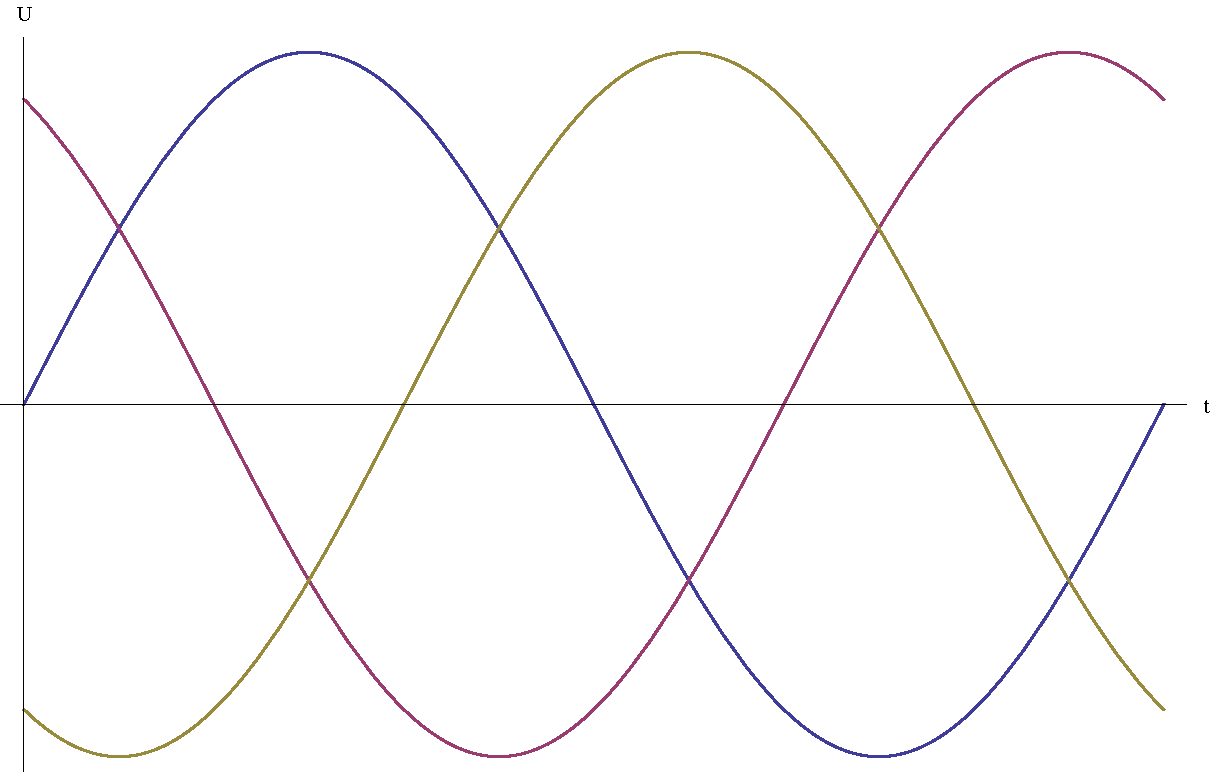
\includegraphics[width=0.5\textwidth]{dreiphasensystem.pdf}
\label{fig:dreiphasensystem}
\caption{Darstellung des Dreiphasensystem mit \textsc{Mathematica}.}
\end{figure}

\section{Einführung Magnetfelder}\label{sec:magnetfelder}

\subsection{Strombelag}\label{sec:strombelag}

Die zeitliche und örtliche Änderung von Magnetfeldern in elektrischen Maschinen wird bestimmt durch die Anordnung stromdurchflossener Leiter und die Art der Speisung \parencite[S.~199]{hofmann2013}.
Die räumliche Verteilung des Stromes wird durch den Strombelag wiedergegeben.
Wenn die Oberfläche eines ferromagnetischen Körpers einen Strombelag $A$ führt, d.\ h.\ wenn eine flächenhafte Strömung vorliegt, liefert das Durchflutungsgesetz

\begin{align}
\oint_{s}{\vec{H}d\vec{s}} = w\cdot I = \Theta \label{durchflutungsgesetz}
\end{align}

$Hds=Ads$, d.\ h.\ $H = A$ bzw.\ $B = \mu A$.
Folgernd existieren neben den Normalkomponenten, $B_n$ und $H_n$ die Tangentialkomponenten $H_t$ und $B_t$ der Feldgrößen.
Die Feldlinien treten nicht mehr senkrecht aus der Randkurve aus, sondern unter einem Winkel $\alpha$.

\begin{align}
\alpha = \arctan(\frac{B_n}{\mu A}) \label{strombelagwinkel}
\end{align}

Der Strombelag wird über dem Umlauf einer Spule bzw.\ Spulengruppe angegeben.

\begin{align}
\Theta(x) = - \int_{x_0}^{x} A(x)dx \label{durchflutung}
\end{align}

damit erhält man durch Differentation den Strombelag $A$

\begin{align}
A(x) = -\partial_x \Theta(x) \label{Strombelag}
\end{align}

mit

\begin{align}
\Theta(x) = \hat{\Theta}(x)\cdot \cos(\frac{\pi}{\tau_p}(x-x_\mu)) \label{adurchflutung}
\end{align}

Nach \ref{durchflutung} ist offensichtlich, dass eine sinusförmige Durchflutungsverteilung nur dann entstehen kann, wenn der Ankerstrombelag ebenfalls sinusförmig, aber um eine Polteilung versetzt ist \parencite[S.~247]{mullerI2005}.

%\begin{figure}[h]
%\centering
%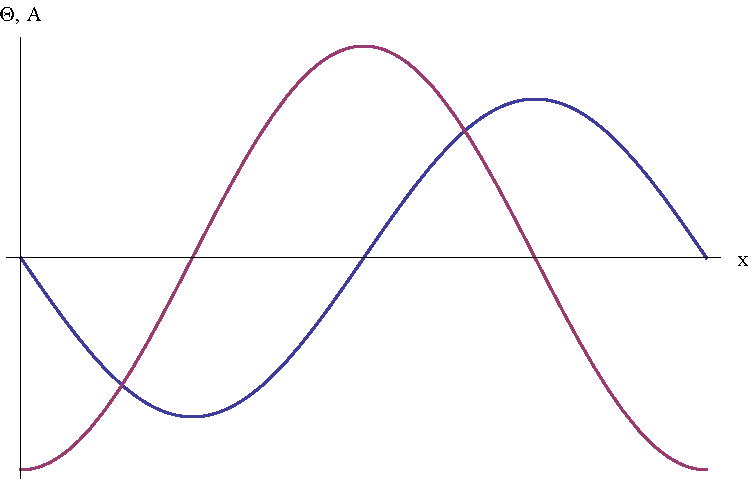
\includegraphics[width=0.5\textwidth]{strombelag.pdf}
%\label{fig:strombelag}
%\caption{Darstellung des sinusförmigen Verlaufs des Strombelags über dem Umlauf.}
%\end{figure}

\section{Allgemeine Grundlagen der Drehstrommaschinen}\label{sec:drehstrommaschinen}

Die Synchron- und Asynchronmaschine besitzen im Ständer denselben Aufbau und erfordern zur Darstellung ihres Verhaltens eine Reihe gleicher physikalischer Begriffe.
Es ist zweckmäßig die Grundlagen der Synchronmaschine in einem eigenen Kapitel zu behandeln.
Dies gilt \insb für den Aufbau der Drehstromwicklungen sowie die Grundlagen zu Beschreibung von umlaufenden Durchflutungen und deren Felder.

\subsection{Drehstromwicklungen}

Der prinzipielle Aufbau einer Drehstromwicklung lässt sich anhand aus den Anforderungen zur Erzeugung einer dreiphasigen Wechselspannung erläutern.
Eine solche Drehspannung erhält man mit einer Anordnung nach \autoref{fig:drehstromwicklung}.
Ein aus Dynamoblechen geschichtetes Ständerblechpacket enthält in Nuten am Bohrungsumfang gleichmäßig verteilte Leiter, die zu drei räumlich verteilten Wicklungssträngen zusammengeschaltet werden \autocite[S.~141]{fischer2009}.
Der Läufer erzeugt ein Gleichfeld, das eine sinusförmige Feldverteilung längst des Luftspaltes aufbaut.
Hat der Läufer eine konstante Drehzahl, so induziert das Feld in den einzelnen Spulen zeitlich sinusförmige Spannungen, die sich innerhalb eines Wicklungsstranges zu einem Wert addieren.
Die Berechnung der Induktion kann über die Allgemeine Beziehung

\begin{align}
u_q = B\cdot l \cdot v
\end{align}

erfolgen.
Sei $d_1$ der Bohrungdurchmesser des Ständerblechpaketes einer $2p$-poligen Maschine, so bezeichnet man den Umfangsanteil

\begin{align}
\tau_p = \frac{d_1 \cdot \pi}{2p}
\end{align}

wieder als Polteilung.
Die Polteilung entspricht der Länder einer Halbwelle der sinusförmigen Flussdichteverteilung im Luftspalt (enspricht einem elektrischen Winkel von $\omega t = 180^{\circ}$.
Bei einer zweipoligen Maschine mit $p=1$ stimmen somit der räumlich mechanische und der elektrische Winkel überein, allgemein gilt die Beziehung \autocite[S.141f.]{fischer2009}

\begin{align}
\gamma_{el} = p\cdot \gamma_{mech}
\end{align}



\begin{figure}[!htb]
\centering
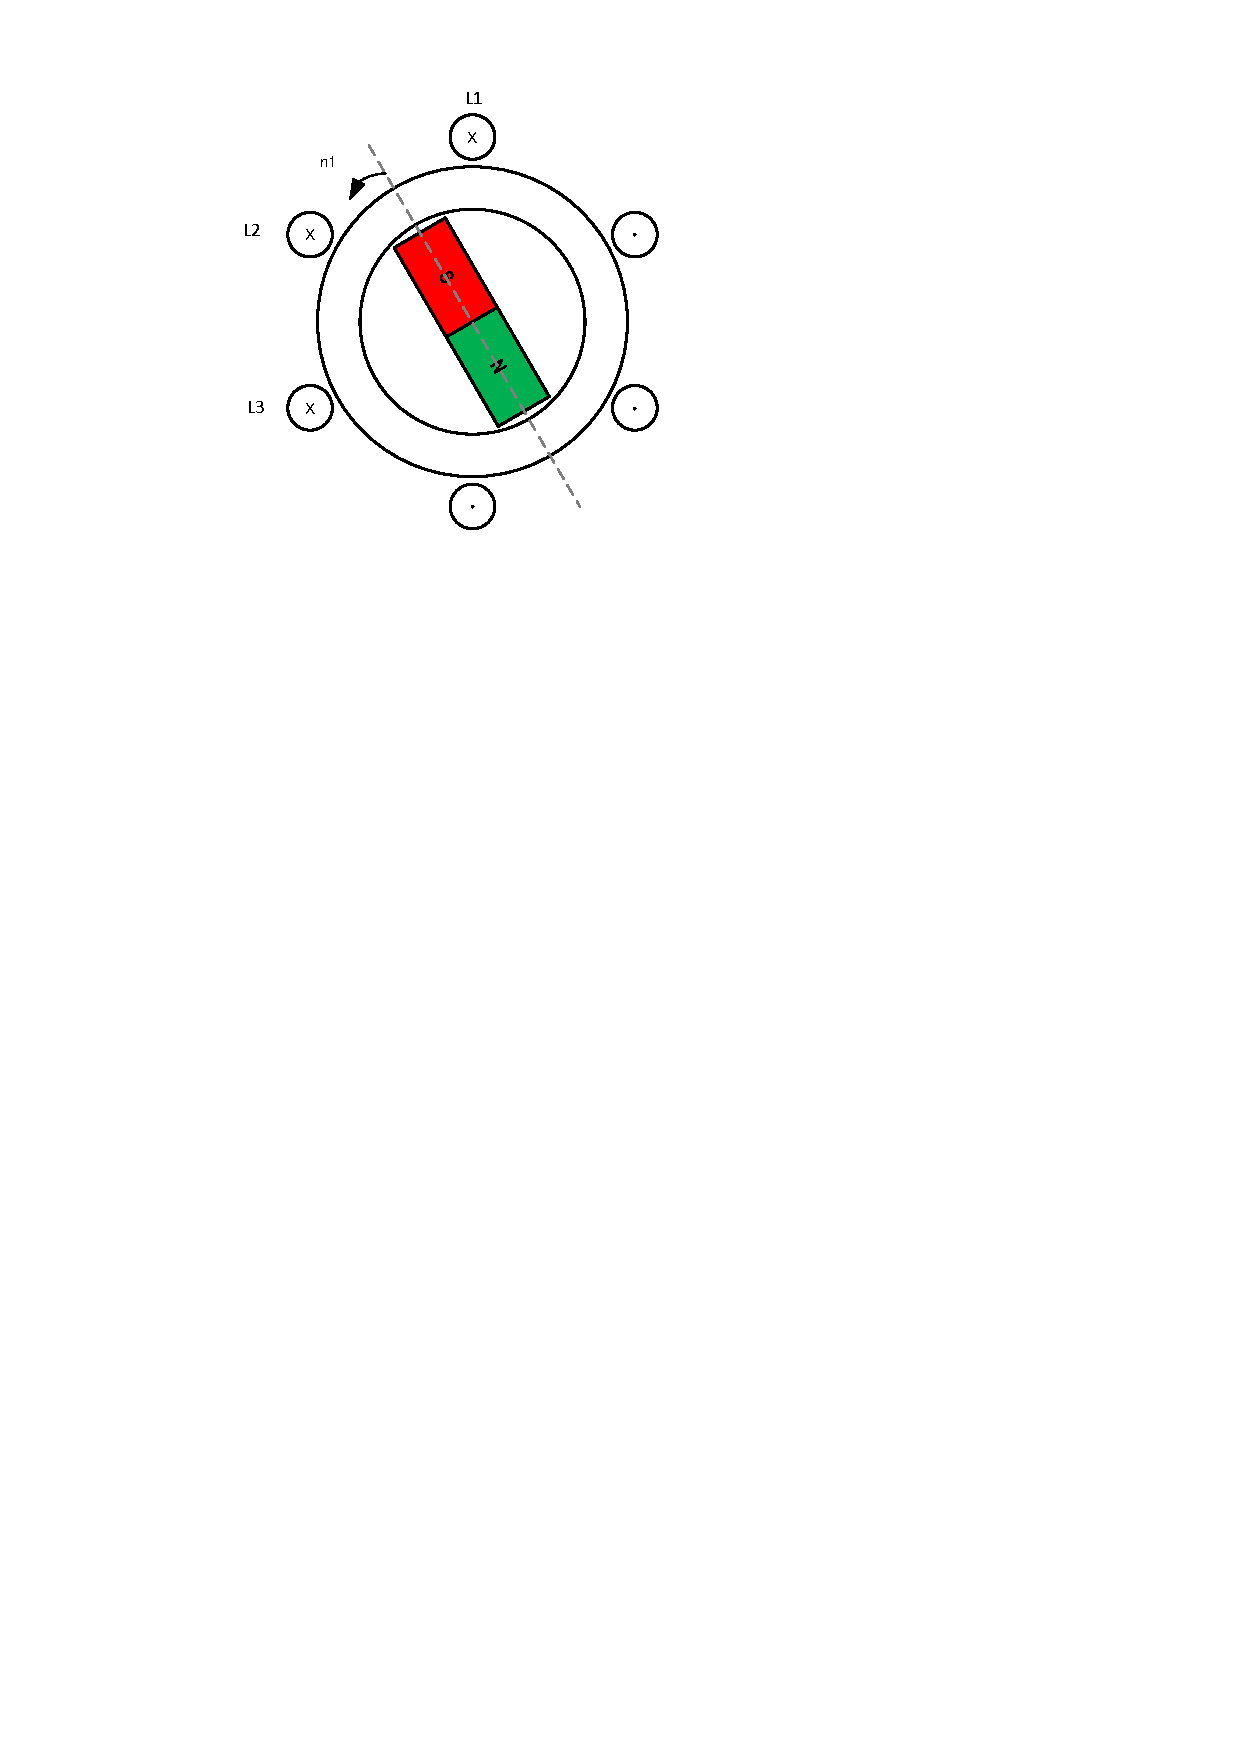
\includegraphics[width=0.5\textwidth]{Visio-synchronmaschine-drehstrom.pdf}
\label{fig:drehstromwicklung}
\caption{Erzeugung einer mehrphasigen Spannung durch ein räumlich sinusförmiges Läuferdrehfeld in Anlehnung an \autocite[S.~141]{fischer2009}}
\end{figure}

\section{Induktivitäten}\label{sec:induktiv}

\section{Einführung Synchronmaschine}\label{sec:synchron}

\section{Permanenterregte Synchronmaschine}\label{sec:pmsm}

\section{Evalurierung der Ersatzschaltbilder für die Regelung}\label{sec:esb}

%%% Local Variables: 
%%% mode: latex
%%% TeX-master: "main"
%%% TeX-open-quote: "\\enquote{"
%%% TeX-close-quote: "}"
%%% LaTeX-csquotes-open-quote: "\\enquote{"
%%% LaTeX-csquotes-close-quote: "}"
%%% End: 

